\section{Câu hỏi 2: Phát hiện ngày và đợt lưu lượng cực trị}
\label{sec:q2}

\subsection{Định nghĩa ngưỡng cực trị}

Báo cáo dùng ngưỡng phân vị 95\% (Q95) của toàn bộ chuỗi 2010--2023 làm định nghĩa
“lưu lượng cao”. Ngưỡng này là \QHigh{} m\textsuperscript{3}/s. Vì Q95 được tính trên
toàn bộ dữ liệu, theo cấu tạo sẽ có khoảng 5\% số ngày vượt ngưỡng. Kết quả thực tế
là \NDaysHigh{} ngày, chiếm \ShareHigh{}\%, rất sát với kỳ vọng.

Có thể chuẩn hóa ngưỡng theo trung bình và độ lệch chuẩn:
\[
z_{95} = \frac{Q95-\bar{Q}}{s_Q}
= \frac{\QHigh-\QMean}{\QStd}
= \ZThreshold.
\]
Giá trị này \emph{không} phải 1,645. Trong phân phối chuẩn, phân vị 95\% tương ứng
với $z \approx 1,645$; nhưng lưu lượng không có phân phối chuẩn và bị lệch. Vì vậy
khi báo cáo nói “ngưỡng Z tĩnh”, cần hiểu đó là cách chuẩn hóa ngưỡng Q95 theo
trung bình và độ lệch chuẩn của chính chuỗi, không phải một kiểm định giả thuyết
phân phối chuẩn. Đây là điểm dễ gây nhầm lẫn nếu chỉ nhìn con số 1,224 mà không
kiểm tra lại định nghĩa.

Một ngày được gọi là “ngày vượt ngưỡng” nếu lưu lượng lớn hơn Q95. Một “đợt” là
dãy ngày vượt ngưỡng liên tiếp; nếu có ít nhất một ngày không vượt ngưỡng ở giữa,
đợt được tách thành hai. Cách định nghĩa này đơn giản, dễ tái lập và phù hợp với
mục tiêu mô tả. Nó không phân biệt mức độ nghiêm trọng giữa các đợt; vì vậy báo cáo
bổ sung số ngày, ngày đỉnh và lưu lượng đỉnh cho từng đợt.

\subsection{Kết quả tổng quan}

Toàn bộ giai đoạn có \NEvents{} đợt vượt ngưỡng. Đợt dài nhất kéo dài
\LongestEvent{} ngày, từ 04/02/2020 đến 03/05/2020, với đỉnh \QMax{}
m\textsuperscript{3}/s vào ngày 10/03/2020. Đợt dài thứ hai kéo dài 77 ngày, từ
13/06/2017 đến 28/08/2017; đợt dài thứ ba kéo dài 61 ngày, từ 15/09/2017 đến
14/11/2017. Ba đợt này chiếm 228 trong tổng số 256 ngày vượt ngưỡng, tức khoảng
89\%.

\begin{table}[H]
\centering
\small
\begin{tabular}{clrrr}
\toprule
Hạng & Khoảng ngày & Số ngày & Ngày đỉnh & Đỉnh (m³/s) \\
\midrule
1 & 04/02/2020–03/05/2020 & 90 & 10/03/2020 & 457{,}49 \\
2 & 13/06/2017–28/08/2017 & 77 & 06/07/2017 & 453{,}52 \\
3 & 15/09/2017–14/11/2017 & 61 & 11/10/2017 & 439{,}97 \\
4 & 02/09/2017–05/09/2017 & 4 & 03/09/2017 & 423{,}71 \\
5 & 13/01/2018–16/01/2018 & 4 & 14/01/2018 & 423{,}21 \\
\bottomrule
\end{tabular}

\caption{Năm đợt lưu lượng cao dài nhất. Danh sách đầy đủ 15 đợt nằm ở phụ lục.}
\label{tab:top-events}
\end{table}

Hình~\ref{fig:extremes-series} đặt ngưỡng Q95 lên toàn bộ chuỗi thời gian. Các đợt
vượt ngưỡng tập trung thành hai cụm lớn: cụm 2017--2018 và cụm 2020. Ngoài hai cụm
này, chỉ có một ngày vượt ngưỡng vào cuối tháng 11/2019. Các năm 2010--2016 và
2021--2023 không có ngày nào vượt Q95. Điều này cho thấy cực trị không phân bố đều
theo thời gian mà phụ thuộc vào những giai đoạn có mức nền cao.

\begin{figure}[H]
\centering
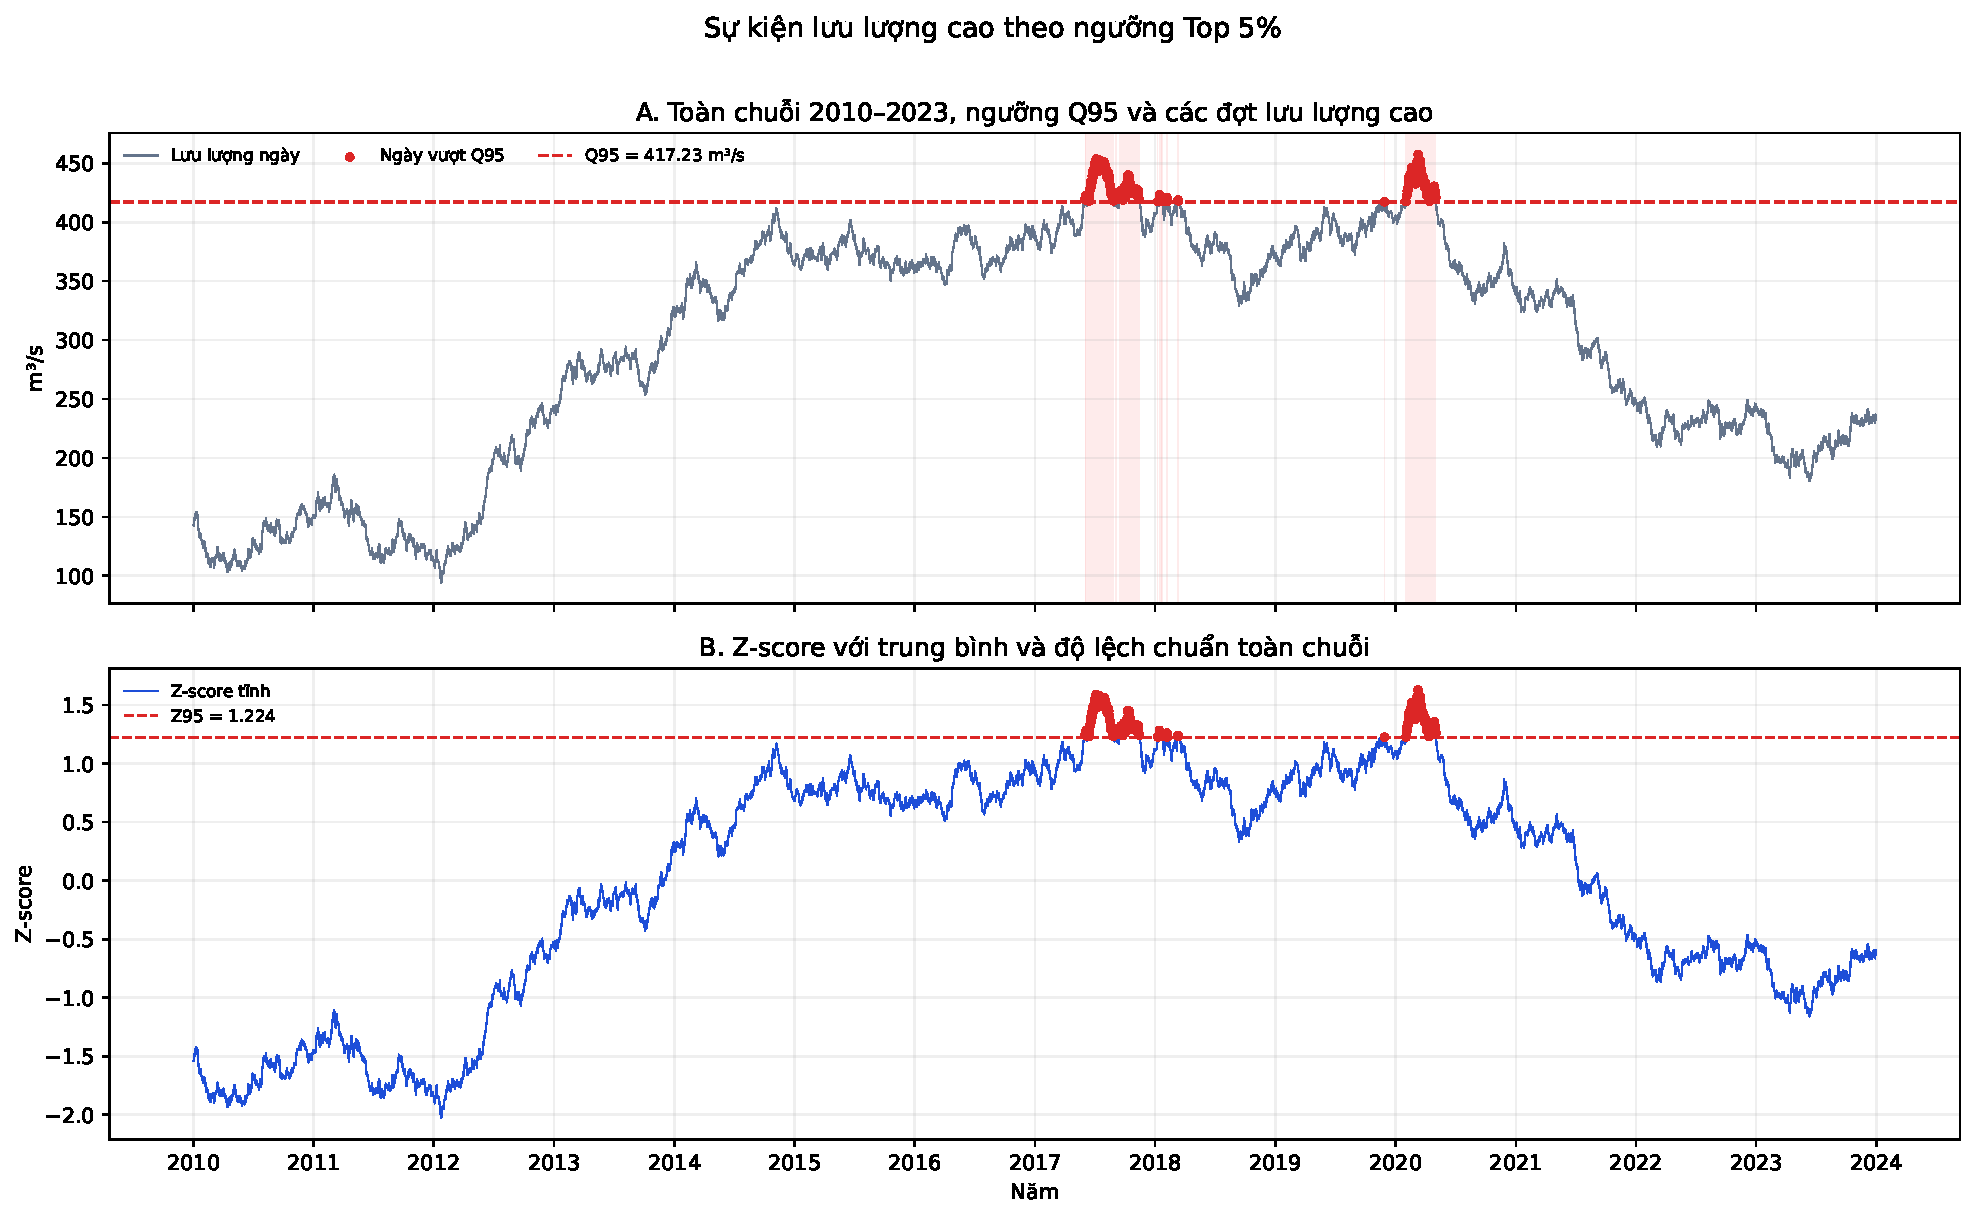
\includegraphics[width=0.96\linewidth]{extremes_full_series.pdf}
\caption{Hai panel: (A) chuỗi lưu lượng và ngưỡng Q95; (B) z-score so với trung bình và độ lệch chuẩn toàn chuỗi. Các điểm vượt ngưỡng tập trung trong 2017--2018 và 2020.}
\label{fig:extremes-series}
\end{figure}

\subsection{Phân bố theo năm}

Bảng~\ref{tab:high-flow-year} cho thấy năm 2017 có 148 ngày vượt ngưỡng, chiếm
40,55\% số ngày của năm và 6 đợt. Năm 2020 có 91 ngày, chiếm 24,86\%, với 2 đợt.
Năm 2018 có 16 ngày, 6 đợt; năm 2019 có 1 ngày, 1 đợt. Tổng cộng 2017 và 2020 chiếm
239/256 ngày vượt ngưỡng, tức hơn 93\%. Sự tập trung này giải thích vì sao các chỉ
số trung bình toàn chuỗi có thể che lấp hành vi cực trị: một vài năm có mức nền cao
chi phối phần lớn số ngày vượt ngưỡng.

\begin{table}[H]
\centering
\small
\begin{tabular}{rrrrr}
\toprule
Năm & Ngày vượt Q95 & Tổng ngày & Tỷ lệ (\%) & Số đợt \\
\midrule
2010 & 0 & 365 & 0{,}00 & 0 \\
2011 & 0 & 365 & 0{,}00 & 0 \\
2012 & 0 & 366 & 0{,}00 & 0 \\
2013 & 0 & 365 & 0{,}00 & 0 \\
2014 & 0 & 365 & 0{,}00 & 0 \\
2015 & 0 & 365 & 0{,}00 & 0 \\
2016 & 0 & 366 & 0{,}00 & 0 \\
2017 & 148 & 365 & 40{,}55 & 6 \\
2018 & 16 & 365 & 4{,}38 & 6 \\
2019 & 1 & 365 & 0{,}27 & 1 \\
2020 & 91 & 366 & 24{,}86 & 2 \\
2021 & 0 & 365 & 0{,}00 & 0 \\
2022 & 0 & 365 & 0{,}00 & 0 \\
2023 & 0 & 365 & 0{,}00 & 0 \\
\bottomrule
\end{tabular}

\caption{Số ngày và số đợt vượt Q95 theo năm.}
\label{tab:high-flow-year}
\end{table}

Năm 2018 đáng chú ý vì có 6 đợt nhưng tổng cộng chỉ 16 ngày. Điều này có nghĩa các
đợt ngắn, bị ngắt bởi những ngày dưới ngưỡng, thay vì một đợt dài. Ngược lại, năm
2020 chỉ có 2 đợt nhưng một đợt kéo dài 90 ngày. Cùng một số ngày vượt ngưỡng có thể
tương ứng với cấu trúc đợt rất khác nhau; vì vậy cần báo cáo cả số ngày và số đợt.

\subsection{Phân bố theo tháng}

Bảng~\ref{tab:high-flow-month} cho thấy các tháng 2, 3, 4 và 10 có số ngày vượt
ngưỡng cao nhất (31, 34, 30 và 31 ngày). Tháng 12 không có ngày nào vượt ngưỡng.
Tuy nhiên, không nên suy ra rằng “mùa lũ” chỉ nằm trong các tháng này, vì các đợt
lớn có thể kéo dài qua nhiều tháng. Đợt 2020 bắt đầu từ tháng 2 và kéo sang tháng 5;
đợt 2017 kéo dài từ tháng 6 đến tháng 11. Vì vậy phân bố theo tháng phản ánh thời
điểm bắt đầu và kết thúc của các đợt, không phản ánh một mùa vụ cố định.

\begin{table}[H]
\centering
\small
\begin{tabular}{rrrr}
\toprule
Tháng & Ngày vượt Q95 & Tổng ngày & Tỷ lệ (\%) \\
\midrule
T1 & 9 & 434 & 2{,}07 \\
T2 & 31 & 395 & 7{,}85 \\
T3 & 34 & 434 & 7{,}83 \\
T4 & 30 & 420 & 7{,}14 \\
T5 & 3 & 434 & 0{,}69 \\
T6 & 24 & 420 & 5{,}71 \\
T7 & 31 & 434 & 7{,}14 \\
T8 & 28 & 434 & 6{,}45 \\
T9 & 20 & 420 & 4{,}76 \\
T10 & 31 & 434 & 7{,}14 \\
T11 & 15 & 420 & 3{,}57 \\
T12 & 0 & 434 & 0{,}00 \\
\bottomrule
\end{tabular}

\caption{Số ngày vượt Q95 theo tháng trên toàn bộ giai đoạn.}
\label{tab:high-flow-month}
\end{table}

\begin{figure}[H]
\centering
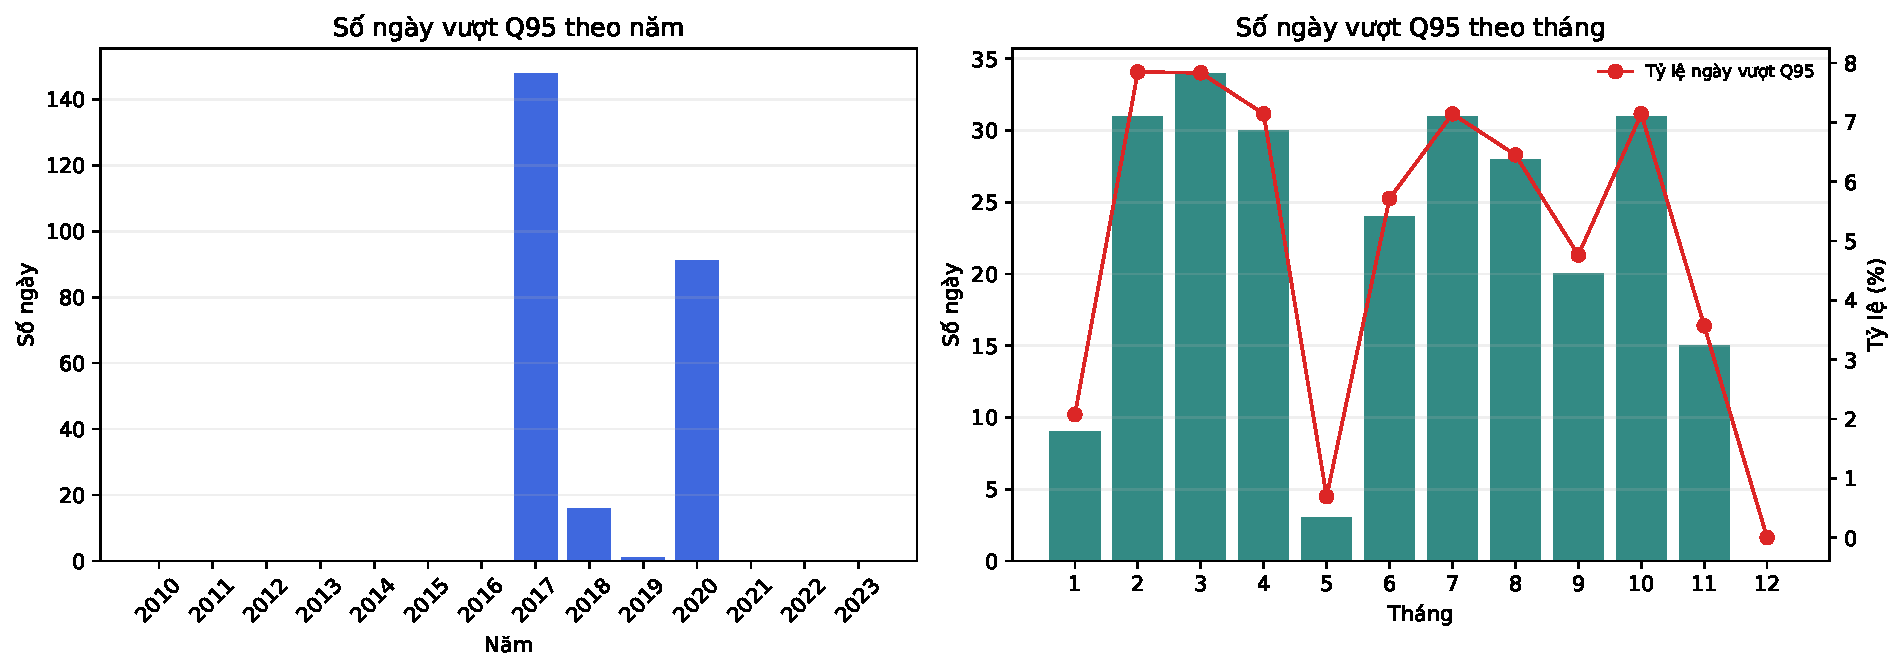
\includegraphics[width=0.9\linewidth]{high_flow_year_month.pdf}
\caption{Bản đồ nhiệt số ngày vượt Q95 theo năm và tháng. Các ô đậm tập trung ở
2017, 2018 và 2020.}
\label{fig:high-flow-heatmap}
\end{figure}

Hình~\ref{fig:high-flow-heatmap} cho thấy rõ hơn cấu trúc theo năm--tháng. Năm 2017
có nhiều ngày vượt ngưỡng từ tháng 6 đến tháng 11; năm 2018 tập trung vào tháng
1--3; năm 2020 tập trung vào tháng 2--5. Đây là các cụm có ý nghĩa thủy văn, không
phải một mùa vụ lặp lại đều đặn. Vì vậy mô hình dự báo cần học từ trạng thái gần
nhất và mức nền hiện tại, thay vì dựa vào mùa vụ lịch.

\subsection{Độ nhạy của ngưỡng}

Ngưỡng Q95 được tính trên toàn bộ chuỗi, không tính lại theo từng năm. Cách làm này
phù hợp cho mục tiêu mô tả “đâu là những ngày cao bất thường so với toàn bộ giai
đoạn”, nhưng có hai giới hạn. Thứ nhất, nếu dùng ngưỡng này để vận hành, ta sẽ dùng
thông tin của tương lai để định nghĩa ngưỡng cho quá khứ. Thứ hai, khi mức nền thay
đổi mạnh, một ngưỡng cố định có thể đánh dấu quá nhiều ngày ở giai đoạn mức cao và
quá ít ngày ở giai đoạn mức thấp.

Một lựa chọn thay thế là ngưỡng trượt theo cửa sổ 365 ngày hoặc ngưỡng theo tháng.
Báo cáo không triển khai các phương án này vì mục tiêu của câu hỏi 2 là mô tả cực
trị toàn giai đoạn, không phải xây dựng hệ thống cảnh báo. Tuy nhiên, đây là hướng
mở rộng tự nhiên nếu dữ liệu được dùng trong vận hành thực tế. Khi đó cần đánh giá
độ nhạy của số đợt, độ dài đợt và đỉnh đợt theo từng cách chọn ngưỡng.

\subsection{Trả lời câu hỏi 2}

Các kết quả chính:

\begin{itemize}[leftmargin=1.4em]
  \item Ngưỡng Q95 là \QHigh{} m\textsuperscript{3}/s, tương ứng z tĩnh
  \ZThreshold{}; có \NDaysHigh{} ngày vượt ngưỡng (\ShareHigh{}\%).
  \item Có \NEvents{} đợt; đợt dài nhất \LongestEvent{} ngày (2020), đợt dài thứ
  hai 77 ngày (2017), đợt dài thứ ba 61 ngày (2017).
  \item Cực trị tập trung vào 2017--2018 và 2020; 2017 và 2020 chiếm hơn 93\% số
  ngày vượt ngưỡng.
  \item Phân bố theo tháng không tạo thành một mùa vụ cố định; các đợt lớn kéo dài
  qua nhiều tháng và phụ thuộc vào mức nền từng năm.
\end{itemize}

Các kết luận này được dùng ở phần dự báo để giải thích vì sao các mô hình có thể
dự báo tốt trung bình nhưng vẫn sai lệch trong các đợt cực trị: cực trị là hiện
tượng hiếm, tập trung theo cụm và chịu ảnh hưởng của mức nền nhiều năm.
